\documentclass[tikz]{standalone}

\usepackage[T1]{fontenc}
\usepackage[utf8]{inputenc}
\usepackage{eulervm}
\usepackage{amsmath}
\usepackage{bm}
\usepackage{tikz}
\usepackage{environ}

\usetikzlibrary{fit}
\usetikzlibrary{patterns}
\usetikzlibrary{arrows}
\usetikzlibrary{shapes.geometric}
\usetikzlibrary{positioning}

\usepackage{color}

\definecolor{Comment}{RGB}{97,161,176}

\definecolor{btfGreen}{RGB}{51,160,44}
\definecolor{btfRed}{RGB}{190,60,90}

\definecolor{bleuUni}{RGB}{0, 157, 224}
\definecolor{marronUni}{RGB}{68, 58, 49}
\definecolor{grayMarronUni}{RGB}{60, 60, 60}
\definecolor{grayBleuUni}{RGB}{118, 118, 118}

\definecolor{bluecite}{HTML}{009DE0}

\definecolor{Paired-2}{RGB}{166,206,227}
\definecolor{Paired-1}{RGB}{31,120,180}
\definecolor{Paired-4}{RGB}{178,223,138}
\definecolor{Paired-3}{RGB}{51,160,44}
\definecolor{Paired-6}{RGB}{251,154,153}
\definecolor{Paired-5}{RGB}{227,26,28}
\definecolor{Paired-8}{RGB}{253,191,111}
\definecolor{Paired-7}{RGB}{255,127,0}
\definecolor{Paired-10}{RGB}{202,178,214}
\definecolor{Paired-9}{RGB}{106,61,154}
\definecolor{Paired-12}{RGB}{255,255,153}
\definecolor{Paired-11}{RGB}{177,89,40}
\definecolor{Accent-1}{RGB}{127,201,127}
\definecolor{Accent-2}{RGB}{190,174,212}
\definecolor{Accent-3}{RGB}{253,192,134}
\definecolor{Accent-4}{RGB}{255,255,153}
\definecolor{Accent-5}{RGB}{56,108,176}
\definecolor{Accent-6}{RGB}{240,2,127}
\definecolor{Accent-7}{RGB}{191,91,23}
\definecolor{Accent-8}{RGB}{102,102,102}
\definecolor{Spectral-1}{RGB}{158,1,66}
\definecolor{Spectral-2}{RGB}{213,62,79}
\definecolor{Spectral-3}{RGB}{244,109,67}
\definecolor{Spectral-4}{RGB}{253,174,97}
\definecolor{Spectral-5}{RGB}{254,224,139}
\definecolor{Spectral-6}{RGB}{255,255,191}
\definecolor{Spectral-7}{RGB}{230,245,152}
\definecolor{Spectral-8}{RGB}{171,221,164}
\definecolor{Spectral-9}{RGB}{102,194,165}
\definecolor{Spectral-10}{RGB}{50,136,189}
\definecolor{Spectral-11}{RGB}{94,79,162}
\definecolor{Set1-1}{RGB}{228,26,28}
\definecolor{Set1-2}{RGB}{55,126,184}
\definecolor{Set1-3}{RGB}{77,175,74}
\definecolor{Set1-4}{RGB}{152,78,163}
\definecolor{Set1-5}{RGB}{255,127,0}
\definecolor{Set1-6}{RGB}{255,255,51}
\definecolor{Set1-7}{RGB}{166,86,40}
\definecolor{Set1-8}{RGB}{247,129,191}
\definecolor{Set1-9}{RGB}{153,153,153}
\definecolor{Set2-1}{RGB}{102,194,165}
\definecolor{Set2-2}{RGB}{252,141,98}
\definecolor{Set2-3}{RGB}{141,160,203}
\definecolor{Set2-4}{RGB}{231,138,195}
\definecolor{Set2-5}{RGB}{166,216,84}
\definecolor{Set2-6}{RGB}{255,217,47}
\definecolor{Set2-7}{RGB}{229,196,148}
\definecolor{Set2-8}{RGB}{179,179,179}
\definecolor{Dark2-1}{RGB}{27,158,119}
\definecolor{Dark2-2}{RGB}{217,95,2}
\definecolor{Dark2-3}{RGB}{117,112,179}
\definecolor{Dark2-4}{RGB}{231,41,138}
\definecolor{Dark2-5}{RGB}{102,166,30}
\definecolor{Dark2-6}{RGB}{230,171,2}
\definecolor{Dark2-7}{RGB}{166,118,29}
\definecolor{Dark2-8}{RGB}{102,102,102}
\definecolor{Reds-1}{RGB}{255,245,240}
\definecolor{Reds-2}{RGB}{254,224,210}
\definecolor{Reds-3}{RGB}{252,187,161}
\definecolor{Reds-4}{RGB}{252,146,114}
\definecolor{Reds-5}{RGB}{251,106,74}
\definecolor{Reds-6}{RGB}{239,59,44}
\definecolor{Reds-7}{RGB}{203,24,29}
\definecolor{Reds-8}{RGB}{165,15,21}
\definecolor{Reds-9}{RGB}{103,0,13}
\definecolor{Greens-1}{RGB}{247,252,245}
\definecolor{Greens-2}{RGB}{229,245,224}
\definecolor{Greens-3}{RGB}{199,233,192}
\definecolor{Greens-4}{RGB}{161,217,155}
\definecolor{Greens-5}{RGB}{116,196,118}
\definecolor{Greens-6}{RGB}{65,171,93}
\definecolor{Greens-7}{RGB}{35,139,69}
\definecolor{Greens-8}{RGB}{0,109,44}
\definecolor{Greens-9}{RGB}{0,68,27}
\definecolor{Blues-1}{RGB}{247,251,255}
\definecolor{Blues-2}{RGB}{222,235,247}
\definecolor{Blues-3}{RGB}{198,219,239}
\definecolor{Blues-4}{RGB}{158,202,225}
\definecolor{Blues-5}{RGB}{107,174,214}
\definecolor{Blues-6}{RGB}{66,146,198}
\definecolor{Blues-7}{RGB}{33,113,181}
\definecolor{Blues-8}{RGB}{8,81,156}
\definecolor{Blues-9}{RGB}{8,48,107}


\begin{document}
  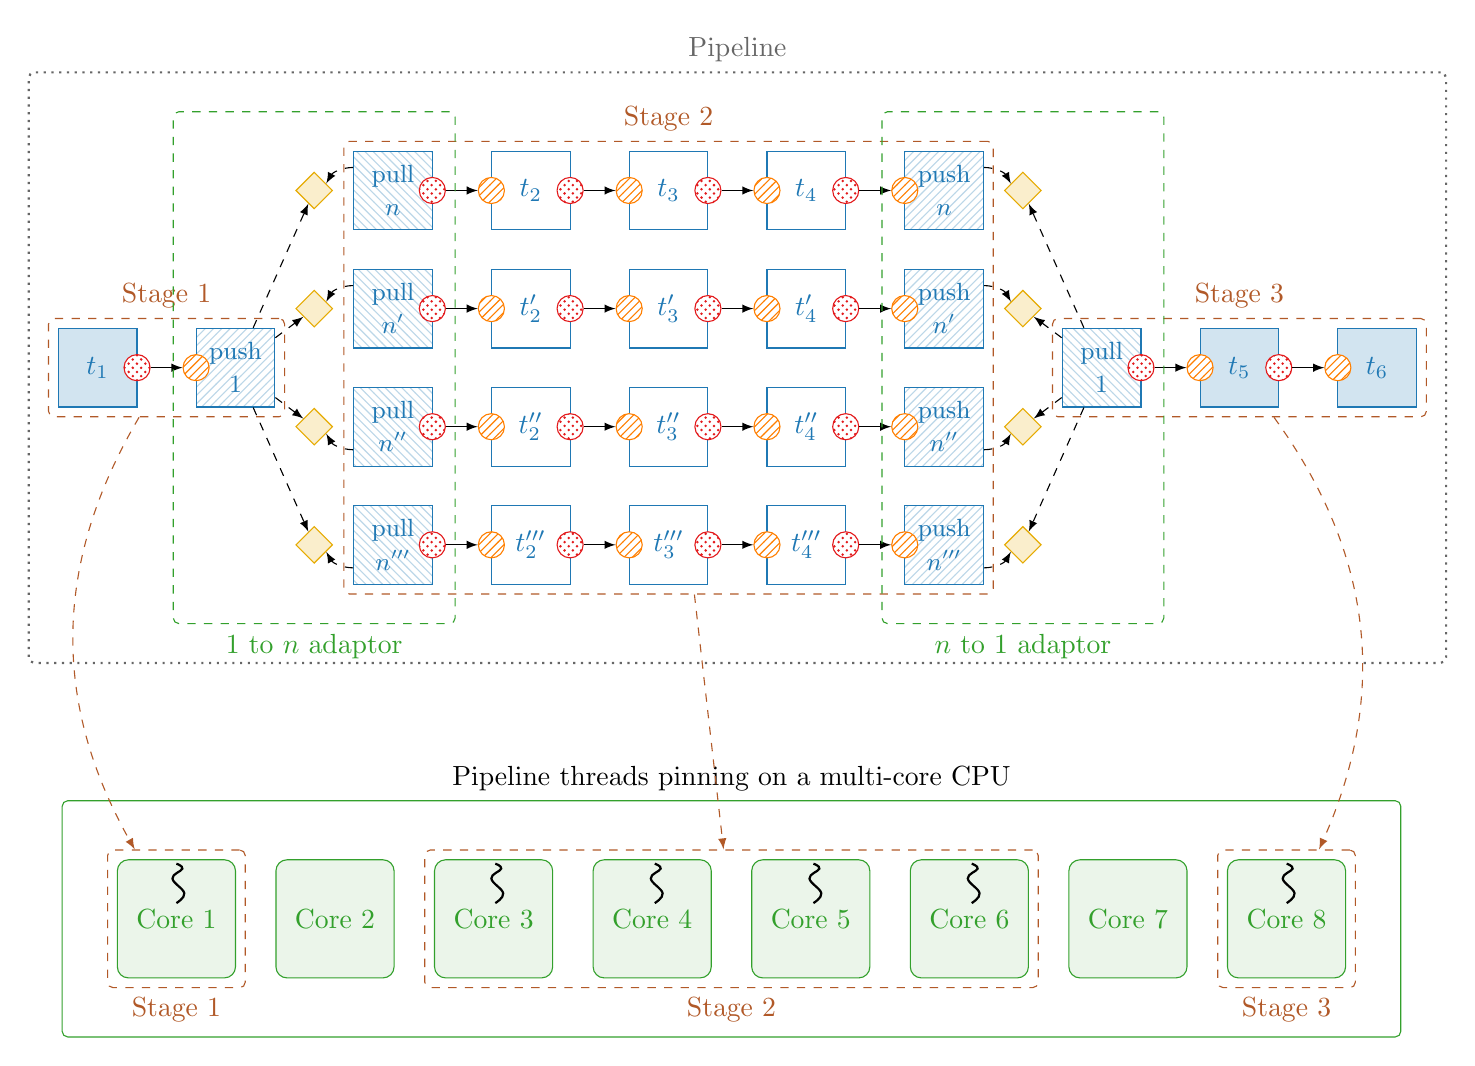
\begin{tikzpicture}%[scale=\tikzscale]
    \tikzset{ tsk/.style ={draw=Paired-1, rounded corners=0pt, text=Paired-1, minimum height=1.0cm, minimum width=1cm} }
    \tikzset{ stsk/.style ={draw=Paired-1, rounded corners=0pt, text=Paired-1, minimum height=1.0cm, minimum width=1cm, fill=Paired-1!20} }
    \tikzset{ push/.style ={draw=Paired-1, align=center, rounded corners=0pt, text=Paired-1, minimum height=1.0cm, minimum width=1cm, preaction={fill=white}, pattern=north east lines, pattern color=Paired-1!30} }
    \tikzset{ pull/.style ={draw=Paired-1, align=center, rounded corners=0pt, text=Paired-1, minimum height=1.0cm, minimum width=1cm, preaction={fill=white}, pattern=north west lines, pattern color=Paired-1!30} }
    \tikzset{ ss/.style  ={draw=Paired-9, rounded corners=2pt, minimum height=1.5cm} }
    \tikzset{ seq/.style ={draw=Paired-11,  dashed, rounded corners=2pt} }
    \tikzset{ mdl/.style ={draw=Paired-3,  dashed, rounded corners=2pt, minimum height=6.5cm} }
    \tikzset{ pip/.style ={draw=Dark2-8,  dotted, thick, rounded corners=2pt} }
    \tikzset{ sin/.style ={draw=Paired-7, circle, minimum width=0.3cm, text=black, preaction={fill=white}, pattern=north east lines, pattern color=Paired-7} }
    \tikzset{ sout/.style={draw=Paired-5, circle, minimum width=0.3cm, text=black, preaction={fill=white}, pattern=crosshatch dots, pattern color=Paired-5} }
    \tikzset{ buff/.style={draw=Dark2-6, diamond, rounded corners=0pt, text=Paired-1, minimum height=0.3cm, minimum width=0.3cm, fill=Dark2-6!20} }

    \newcommand{\thread}[3]{
      \draw[thick, xshift=#1cm, yshift=#2cm] plot [smooth,tension=0.7] coordinates {(0,0.5) (0.075,0.4375) (-0.05,0.3125) (0.1,0.125) (0,0)} node (#3){};
    }

    \node[stsk] (t1)    at ( 0.0    , 0.0) {$t_1$};
    \node[sout] (t1_so) at ( 0.0+0.5, 0.0) {};

    \node[push] (adp1n_push)    at ( 1.75    , 0.0) {\small{push}\\\small{$1$}};
    \node[sin ] (adp1n_push_si) at ( 1.75-0.5, 0.0) {};

    \newcommand\thr{+2.25}
    \node[buff] (adp1n_b1)       at ( 2.75    , \thr) {};
    \node[pull] (adp1n_pull1)    at ( 3.75    , \thr) {\small{pull}\\\small{$n$}};
    \node[sout] (adp1n_pull1_so) at ( 3.75+0.5, \thr) {};
    \node[tsk ] (t2)             at ( 5.50    , \thr) {$t_2$};
    \node[sin ] (t2_si)          at ( 5.50-0.5, \thr) {};
    \node[sout] (t2_so)          at ( 5.50+0.5, \thr) {};
    \node[tsk ] (t3)             at ( 7.25    , \thr) {$t_3$};
    \node[sin ] (t3_si)          at ( 7.25-0.5, \thr) {};
    \node[sout] (t3_so)          at ( 7.25+0.5, \thr) {};
    \node[tsk ] (t4)             at ( 9.00    , \thr) {$t_4$};
    \node[sin ] (t4_si)          at ( 9.00-0.5, \thr) {};
    \node[sout] (t4_so)          at ( 9.00+0.5, \thr) {};
    \node[push] (adpn1_push1)    at (10.75    , \thr) {\small{push}\\\small{$n$}};
    \node[sin ] (adpn1_push1_si) at (10.75-0.5, \thr) {};
    \node[buff] (adpn1_b1)       at (11.75    , \thr) {};

    \draw[->,>=latex] (adp1n_pull1_so) -- (t2_si) node [midway, above] {};
    \draw[->,>=latex] (t2_so)          -- (t3_si) node [midway, above] {};
    \draw[->,>=latex] (t3_so)          -- (t4_si) node [midway, above] {};
    \draw[->,>=latex] (t4_so)          -- (adpn1_push1_si) node [midway, above] {};

    \newcommand\tthr{+0.75}
    \node[buff] (adp1n_b2)       at ( 2.75    , \tthr) {};
    \node[pull] (adp1n_pull2)    at ( 3.75    , \tthr) {\small{pull}\\\small{$n'$}};
    \node[sout] (adp1n_pull2_so) at ( 3.75+0.5, \tthr) {};
    \node[tsk ] (tt2)            at ( 5.50    , \tthr) {$t_2'$};
    \node[sin ] (tt2_si)         at ( 5.50-0.5, \tthr) {};
    \node[sout] (tt2_so)         at ( 5.50+0.5, \tthr) {};
    \node[tsk ] (tt3)            at ( 7.25    , \tthr) {$t_3'$};
    \node[sin ] (tt3_si)         at ( 7.25-0.5, \tthr) {};
    \node[sout] (tt3_so)         at ( 7.25+0.5, \tthr) {};
    \node[tsk ] (tt4)            at ( 9.00    , \tthr) {$t_4'$};
    \node[sin ] (tt4_si)         at ( 9.00-0.5, \tthr) {};
    \node[sout] (tt4_so)         at ( 9.00+0.5, \tthr) {};
    \node[push] (adpn1_push2)    at (10.75    , \tthr) {\small{push}\\\small{$n'$}};
    \node[sin ] (adpn1_push2_si) at (10.75-0.5, \tthr) {};
    \node[buff] (adpn1_b2)       at (11.75    , \tthr) {};

    \draw[->,>=latex] (adp1n_pull2_so) -- (tt2_si) node [midway, above] {};
    \draw[->,>=latex] (tt2_so)         -- (tt3_si) node [midway, above] {};
    \draw[->,>=latex] (tt3_so)         -- (tt4_si) node [midway, above] {};
    \draw[->,>=latex] (tt4_so)         -- (adpn1_push2_si) node [midway, above] {};

    \newcommand\ttthr{-0.75}
    \node[buff] (adp1n_b3)       at ( 2.75    , \ttthr) {};
    \node[pull] (adp1n_pull3)    at ( 3.75    , \ttthr) {\small{pull}\\\small{$n''$}};
    \node[sout] (adp1n_pull3_so) at ( 3.75+0.5, \ttthr) {};
    \node[tsk ] (ttt2)           at ( 5.50    , \ttthr) {$t_2''$};
    \node[sin ] (ttt2_si)        at ( 5.50-0.5, \ttthr) {};
    \node[sout] (ttt2_so)        at ( 5.50+0.5, \ttthr) {};
    \node[tsk ] (ttt3)           at ( 7.25    , \ttthr) {$t_3''$};
    \node[sin ] (ttt3_si)        at ( 7.25-0.5, \ttthr) {};
    \node[sout] (ttt3_so)        at ( 7.25+0.5, \ttthr) {};
    \node[tsk ] (ttt4)           at ( 9.00    , \ttthr) {$t_4''$};
    \node[sin ] (ttt4_si)        at ( 9.00-0.5, \ttthr) {};
    \node[sout] (ttt4_so)        at ( 9.00+0.5, \ttthr) {};
    \node[push] (adpn1_push3)    at (10.75    , \ttthr) {\small{push}\\\small{$n''$}};
    \node[sin ] (adpn1_push3_si) at (10.75-0.5, \ttthr) {};
    \node[buff] (adpn1_b3)       at (11.75    , \ttthr) {};

    \draw[->,>=latex] (adp1n_pull3_so) -- (ttt2_si) node [midway, above] {};
    \draw[->,>=latex] (ttt2_so)        -- (ttt3_si) node [midway, above] {};
    \draw[->,>=latex] (ttt3_so)        -- (ttt4_si) node [midway, above] {};
    \draw[->,>=latex] (ttt4_so)        -- (adpn1_push3_si) node [midway, above] {};

    \newcommand\tttthr{-2.25}
    \node[buff] (adp1n_b4)       at ( 2.75    , \tttthr) {};
    \node[pull] (adp1n_pull4)    at ( 3.75    , \tttthr) {\small{pull}\\\small{$n'''$}};
    \node[sout] (adp1n_pull4_so) at ( 3.75+0.5, \tttthr) {};
    \node[tsk ] (tttt2)          at ( 5.50    , \tttthr) {$t_2'''$};
    \node[sin ] (tttt2_si)       at ( 5.50-0.5, \tttthr) {};
    \node[sout] (tttt2_so)       at ( 5.50+0.5, \tttthr) {};
    \node[tsk ] (tttt3)          at ( 7.25    , \tttthr) {$t_3'''$};
    \node[sin ] (tttt3_si)       at ( 7.25-0.5, \tttthr) {};
    \node[sout] (tttt3_so)       at ( 7.25+0.5, \tttthr) {};
    \node[tsk ] (tttt4)          at ( 9.00    , \tttthr) {$t_4'''$};
    \node[sin ] (tttt4_si)       at ( 9.00-0.5, \tttthr) {};
    \node[sout] (tttt4_so)       at ( 9.00+0.5, \tttthr) {};
    \node[push] (adpn1_push4)    at (10.75    , \tttthr) {\small{push}\\\small{$n'''$}};
    \node[sin ] (adpn1_push4_si) at (10.75-0.5, \tttthr) {};
    \node[buff] (adpn1_b4)       at (11.75    , \tttthr) {};

    \draw[->,>=latex] (adp1n_pull4_so) -- (tttt2_si) node [midway, above] {};
    \draw[->,>=latex] (tttt2_so)       -- (tttt3_si) node [midway, above] {};
    \draw[->,>=latex] (tttt3_so)       -- (tttt4_si) node [midway, above] {};
    \draw[->,>=latex] (tttt4_so)       -- (adpn1_push4_si) node [midway, above] {};

    \node[pull] (adpn1_pull)    at (12.75    , 0.0) {\small{pull}\\\small{$1$}};
    \node[sout] (adpn1_pull_so) at (12.75+0.5, 0.0) {};
    \node[stsk] (t5)            at (14.50    , 0.0) {$t_5$};
    \node[sin ] (t5_si)         at (14.50-0.5, 0.0) {};
    \node[sout] (t5_so)         at (14.50+0.5, 0.0) {};
    \node[stsk] (t6)            at (16.25    , 0.0) {$t_6$};
    \node[sin ] (t6_si)         at (16.25-0.5, 0.0) {};

    \draw[->,>=latex] (t1_so)         -- (adp1n_push_si) node [midway, above] {};
    \draw[->,>=latex] (adpn1_pull_so) -- (t5_si) node [midway, above] {};
    \draw[->,>=latex] (t5_so)         -- (t6_si) node [midway, above] {};

    \draw[->,>=latex,dashed] (adp1n_push) -- (adp1n_b1) node [midway, above] {};
    \draw[->,>=latex,dashed] (adp1n_push) -- (adp1n_b2) node [midway, above] {};
    \draw[->,>=latex,dashed] (adp1n_push) -- (adp1n_b3) node [midway, above] {};
    \draw[->,>=latex,dashed] (adp1n_push) -- (adp1n_b4) node [midway, above] {};

    \draw[->,>=latex,dashed] (adpn1_pull) -- (adpn1_b1) node [midway, above] {};
    \draw[->,>=latex,dashed] (adpn1_pull) -- (adpn1_b2) node [midway, above] {};
    \draw[->,>=latex,dashed] (adpn1_pull) -- (adpn1_b3) node [midway, above] {};
    \draw[->,>=latex,dashed] (adpn1_pull) -- (adpn1_b4) node [midway, above] {};

    \draw[->,>=latex,dashed] (adp1n_pull1) to[bend right] (adp1n_b1) node [midway, above] {};
    \draw[->,>=latex,dashed] (adp1n_pull2) to[bend right] (adp1n_b2) node [midway, above] {};
    \draw[->,>=latex,dashed] (adp1n_pull3) to[bend  left] (adp1n_b3) node [midway, above] {};
    \draw[->,>=latex,dashed] (adp1n_pull4) to[bend  left] (adp1n_b4) node [midway, above] {};

    \draw[->,>=latex,dashed] (adpn1_push1) to[bend  left] (adpn1_b1) node [midway, above] {};
    \draw[->,>=latex,dashed] (adpn1_push2) to[bend  left] (adpn1_b2) node [midway, above] {};
    \draw[->,>=latex,dashed] (adpn1_push3) to[bend right] (adpn1_b3) node [midway, above] {};
    \draw[->,>=latex,dashed] (adpn1_push4) to[bend right] (adpn1_b4) node [midway, above] {};

    \node[seq, label={[Paired-11]above:Stage 1}, fit=(t1) (t1_so) (adp1n_push)  ] (seq1) {};
    \node[seq, label={[Paired-11]above:Stage 2}, fit=(adp1n_pull1) (adpn1_push4)] (seq2) {};
    \node[seq, label={[Paired-11]above:Stage 3}, fit=(adpn1_pull) (t5) (t6)     ] (seq3) {};

    \node[mdl, label={[Paired-3]below:$1$ to $n$ adaptor}, fit=(adp1n_push_si) (adp1n_pull1) (adp1n_pull1_so) (adp1n_pull4) (adp1n_pull4_so)] (adp1n) {};
    \node[mdl, label={[Paired-3]below:$n$ to $1$ adaptor}, fit=(adpn1_pull_so) (adpn1_push1) (adpn1_push1_si) (adpn1_push4) (adpn1_push4_si)] (adpn1) {};

    \node[pip, minimum height=2.5cm, minimum width=18.0cm, minimum height=7.5cm, label={[Dark2-8]above:Pipeline}, fit=(seq1) (seq2) (seq3) (adp1n) (adpn1)] {};

    \tikzset{ core/.style ={ draw=Paired-3, fill=Paired-3!10, minimum width=1.5cm, minimum height=1.5cm, text=Paired-3, rounded corners=4pt } }
    \tikzset{ cpu/.style ={ draw=Paired-3, rounded corners=2pt } }

    \node[core                    ] (c1) at (1.0, -7.0) {Core 1};
    \node[core, right=0.50cm of c1] (c2)                {Core 2};
    \node[core, right=0.50cm of c2] (c3)                {Core 3};
    \node[core, right=0.50cm of c3] (c4)                {Core 4};
    \node[core, right=0.50cm of c4] (c5)                {Core 5};
    \node[core, right=0.50cm of c5] (c6)                {Core 6};
    \node[core, right=0.50cm of c6] (c7)                {Core 7};
    \node[core, right=0.50cm of c7] (c8)                {Core 8};

    \node[seq, label={[Paired-11]below:Stage 1}, fit=(c1)     ] (sta1) {};
    \node[seq, label={[Paired-11]below:Stage 2}, fit=(c3) (c6)] (sta2) {};
    \node[seq, label={[Paired-11]below:Stage 3}, fit=(c8)     ] (sta3) {};

    \node[cpu, minimum height=3.0cm, minimum width=17.0cm, label={[black]above:Pipeline threads pinning on a multi-core CPU}, fit=(c1) (c8)] {};

    \thread{ 1.000}{-6.8}{th1}
    \thread{ 5.050}{-6.8}{th2}
    \thread{ 7.075}{-6.8}{th3}
    \thread{ 9.090}{-6.8}{th4}
    \thread{11.100}{-6.8}{th5}
    \thread{15.100}{-6.8}{th6}

    \draw[->,>=latex,dashed, draw=Paired-11] (seq1) to[bend  right] (sta1) node [midway, above] {};
    \draw[->,>=latex,dashed, draw=Paired-11] (seq2) --              (sta2) node [midway, sloped] {};
    \draw[->,>=latex,dashed, draw=Paired-11] (seq3) to[bend  left]  (sta3) node [midway, above] {};


  \end{tikzpicture}
\end{document}